
\documentclass[letter, 9pt, conference]{ieeeconf}

\IEEEoverridecommandlockouts

\overrideIEEEmargins

\usepackage[utf8]{inputenc}
\usepackage[T1]{fontenc}
%\usepackage[top=0.75in, bottom=1in, left=1in, right=1in]{geometry}
\usepackage{xcolor}
\usepackage{graphicx}
\usepackage{hyperref}

\title{Project report - OVH topology}

\author{Langlois Quentin - 19-28-1700 \and Dardenne Florent - 02-60-1700 \and Iavarone Simon xx-xx-xxxx }


\begin{document}

\maketitle
\thispagestyle{empty}
\pagestyle{empty}


%%%%%%%%%%%%%%%%%%%%%%%%%%%%%%%%%%%%%%%%%%%%%%%%%%%%%%%%%%%%%%%%%%%%%%%%%%%%%%%%
\begin{abstract}

This report will describe our analyze of the East-Europa OVH network topology. It will detail different aspects such as oSPF, BGP, security and anycast. At the end, we will present our simulation technique, tests and results. 

\end{abstract}


%%%%%%%%%%%%%%%%%%%%%%%%%%%%%%%%%%%%%%%%%%%%%%%%%%%%%%%%%%%%%%%%%%%%%%%%%%%%%%%%
\section{Introduction}

For this project, we were asked to choose a part of the OVH topology, describe and simulate it with the \textbf{ipmininet} library. 

This report will first describe the part of the topology we chose and some information about it such as OSPF and BGP. 

Next, we will present 3 additional aspects such as security, BGP communities and anycast. 

Finally, we will show our simulation methodology, tests and results. 

\section{Description of the topology}

\subsection{Zone description}

We chose the East-Europa zone of the topology. This choice was done for 2 reasons : 

\begin{itemize}
    \item There are many redundancies in this part of the network. 
    \item Many external ASes are present at many places which allows us to more interesting simulation of the eBGP mechanism. 
\end{itemize}

\begin{figure}[h!]
    \includegraphics[width=\linewidth]{topo_schema.jpeg}
    \caption{Topology representation}
    \label{fig:topo_schema}
\end{figure}

Legend : 
\begin{itemize}
    \item Boxes represents routers and their color represents their AS (one color per AS). 
    \item Links represents physical links with their associated IGP cost\footnote{Seep section \ref{sec:ibgp} for more details} (1 by default). 
    \item Circles represents a group of Route-Reflector. 
\end{itemize}



\subsection{OSPF and addressing plan}
\label{sec:ospf}

In order to safe a maximum of IP addresses, we chose a \textbf{hierarchical adressing} plan. 

For this purpose, we first assigned a specific subnet for each AS (in /24 for IPv4 and /48 for IPv6). 

Next, we divided the OVH network by region (cities) and gave them a more specific subnet (in /28 for IPv4 and /56 for IPv6). 

The last step was to determine the loopback-address of routers and the address of their interfaces for link addresses. As described in the section \ref{sec:simulation}, we made an incremental address generator for loopback-address and use the same technique for link-addressing. \\
This means we took the first available address (in /32 or /128 for loopback) and assign it to the router. For the links, we choose the subnet of one of the two routers and generate 2 addresses (in /31 or /127) in order to put the 2 routers in the same subnet. 


\subsection{iBGP configuration}
\label{sec:ibgp}

In order to have a minimal number of iBGP connections, we chose a multi-level Route-Reflector (RR) architecture. 

Furthermore, as shown in the \ref{fig:ibgp_schema}, the iBGP connections follows, in majority cases, physical links connections. 

In order to make redundancy, all routers are connected to at least two Route-Reflectors. 

IGP costs allows to avoid diflection also in case of crashes. 

\begin{figure}[h!]
    \includegraphics[width=\linewidth]{ibgp_schema.jpeg}
    \caption{iBGP connections}
    \label{fig:ibgp_schema}
\end{figure}

Description of the RR-levels : 
\begin{itemize}
    \item \textbf{First level} : main level which will dispatch routes to second-level-RR. \\
    We chose \textit{fra-5} and \textit{par-gsw} because they are connected to many other ASes and then have a central positions and recieve many external routes. 
    \item \textbf{Second level} : we splitted the second-level RR in 2 sub-groups : 
    \begin{itemize}
        \item At the left of the topology (with \textit{milan} and \textit{sbg-g1} which will dispatch routes to this part. 
        \item \textit{ams-5}, \textit{vienne} and \textit{varsovie} which will dispatch routes to the left part of the topology. 
    \end{itemize}
    A fullmesh is done for each subgroups. 
\end{itemize}

\subsection{eBGP configuration}
\label{sec:ebgp}

In order to have a more realistic topology, we had decided to add 1 external AS router for each connection with OVH. Indeed, 1 router connected to Milan, Warsow, Amsterdam,Paris and Frankfurt (for UPC) seemed not realistic at all. 

We chose to make \textbf{client-provider sessions} (where OVH is the provider) as we considered OVH as a transit network. 

\subsection{Topology summary}
\label{sec:summary}

As described in the \ref{sec:simulation} section, we also added methods to print statistics on the topology. Here is a screen of the result. 

\begin{figure}[h!]
    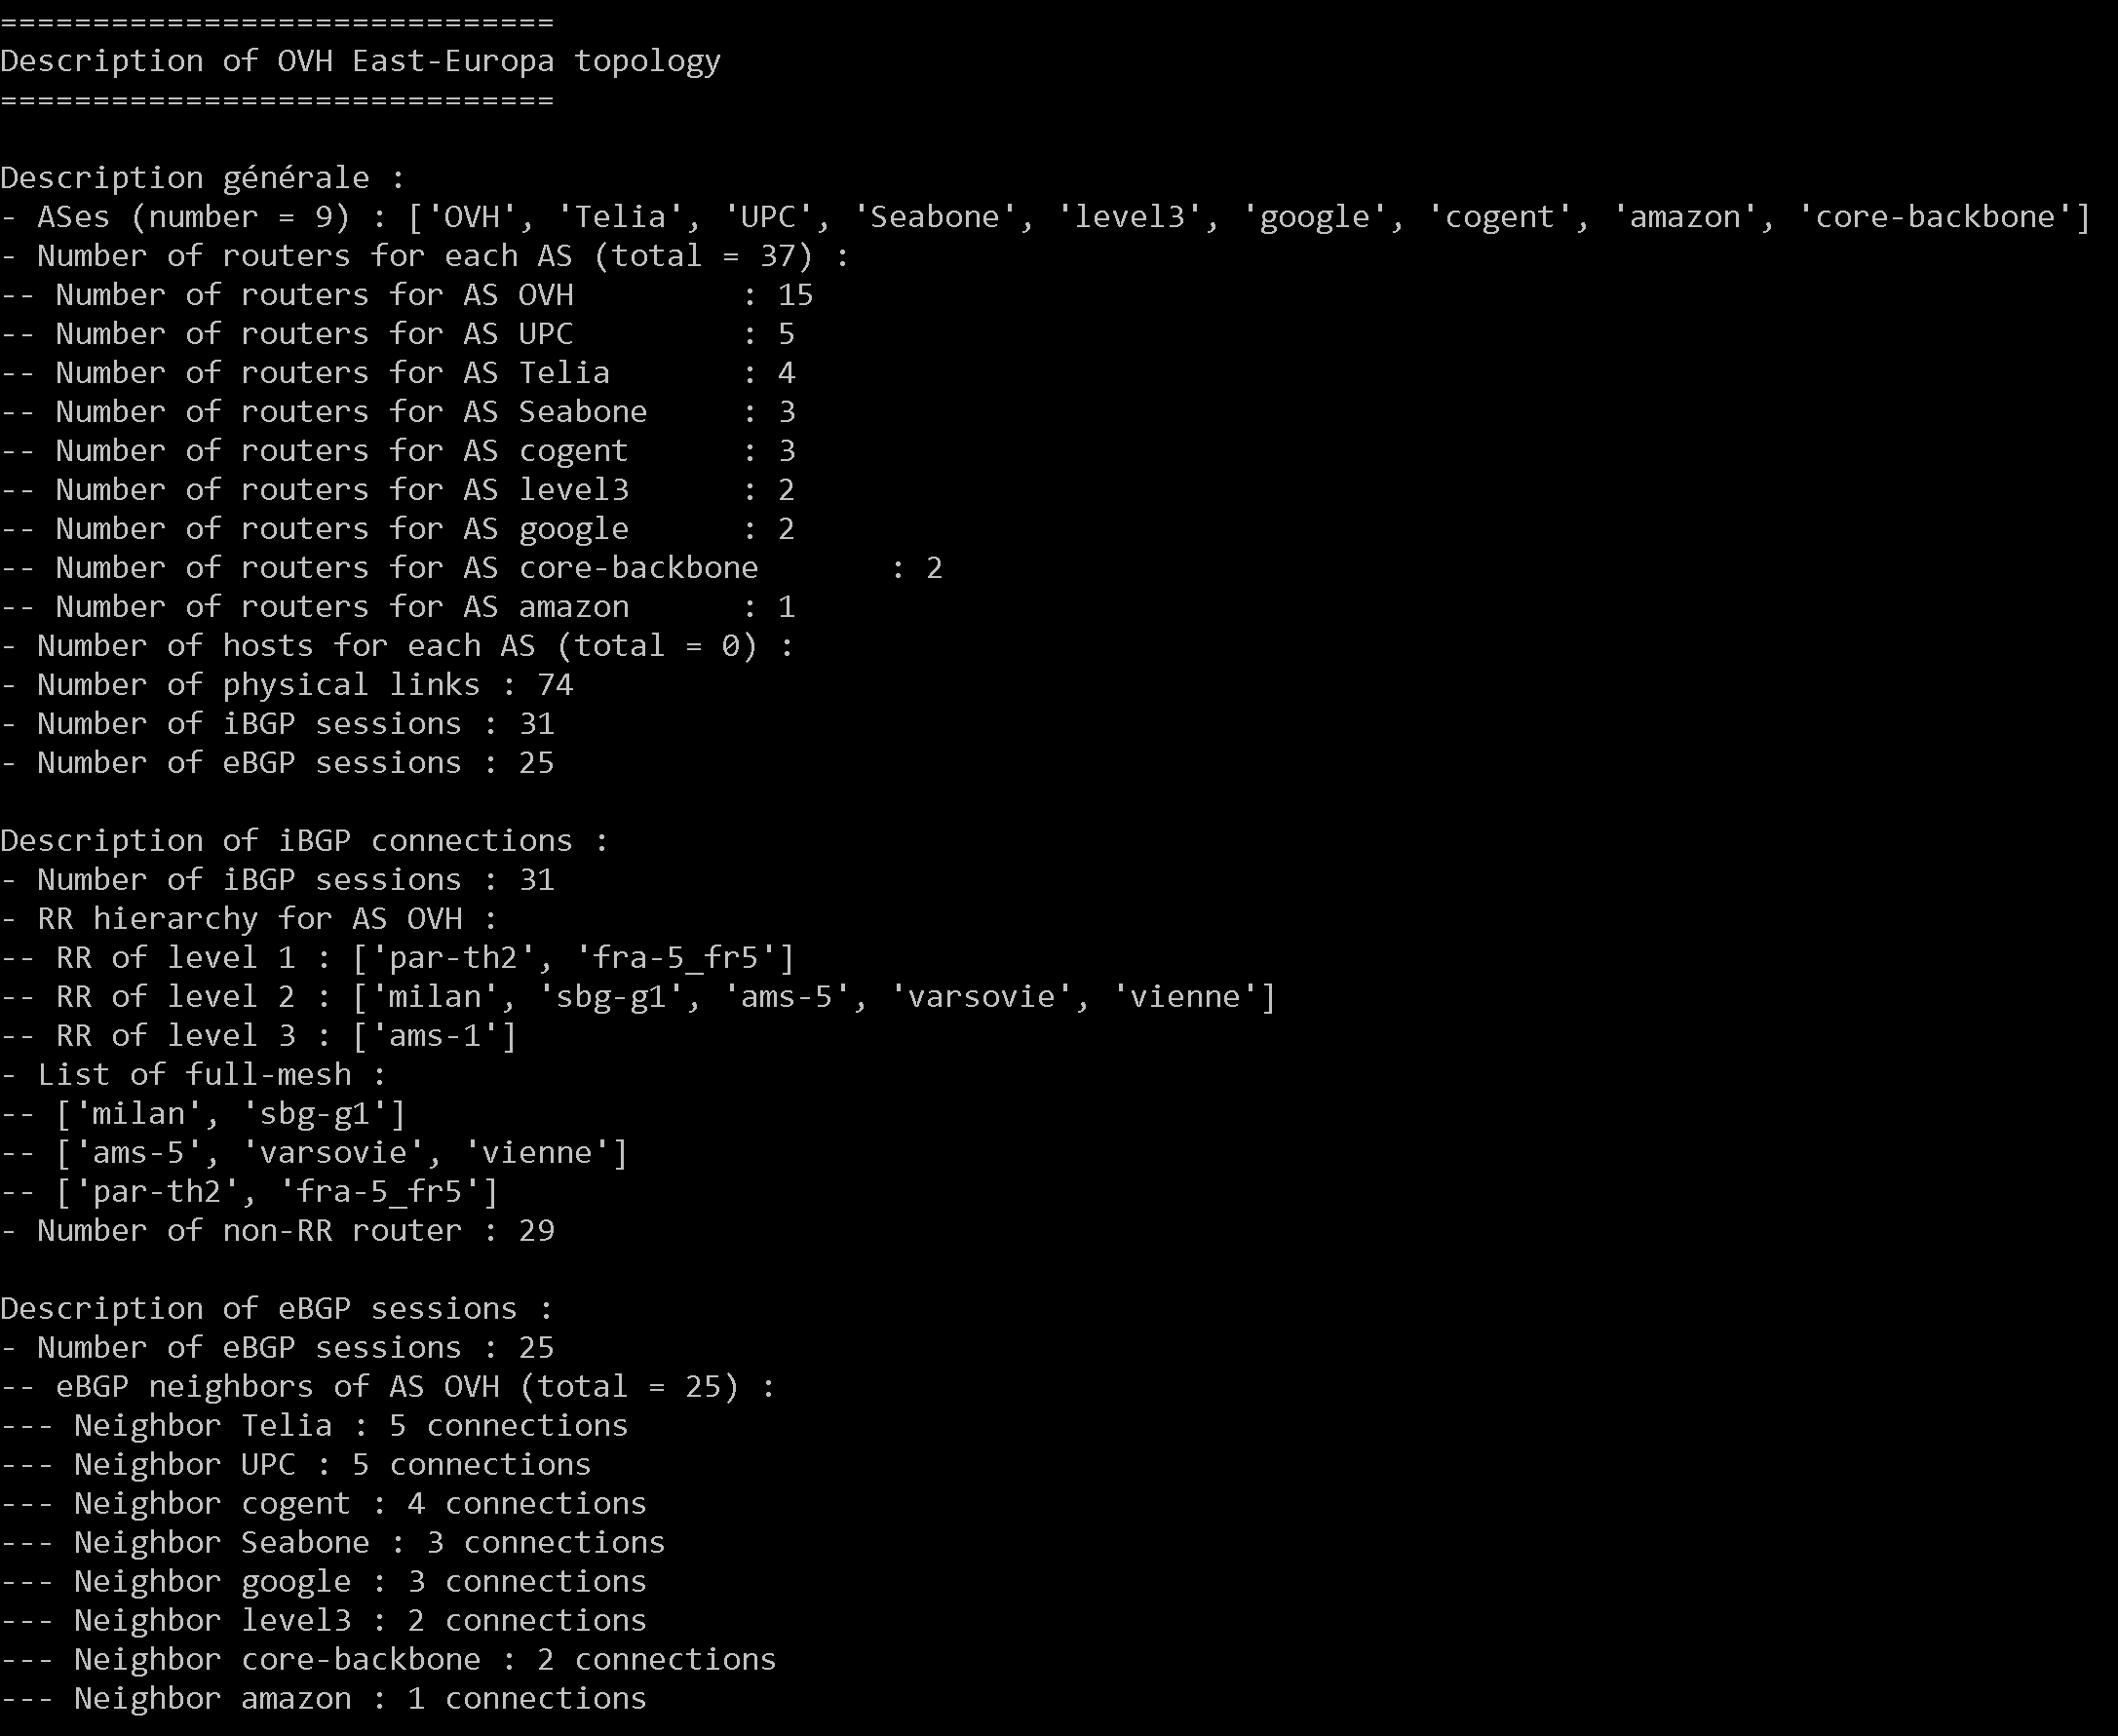
\includegraphics[width=\linewidth]{topo_summary.PNG}
    \caption{Information about the topology}
    \label{fig:topo_summary}
\end{figure}


\section{Security}
\label{sec:security}


\section{BGP communities}
\label{sec:communities}


\section{Anycast}
\label{sec:anycast}

\subsection{Anycast techniques}

Anycast is the ability to have multiple \textbf{servers} with the sime IP address in a network and join the nearest from its position. 

There are many possible utilization for this feature such as DNS servers, data-centers, ... 

In order to configure anycast, there are 3 main ways : 
\begin{itemize}
    \item \textbf{DNS zones} : groups some servers under a unique domain name. 
    \item \textbf{OSPF} : advertise multiple times the same IP address over OSPF. 
    \item \textbf{BGP} : advertise multiple times the same IP address over BGP. 
\end{itemize}

\subsection{Anycast in our topology}

For this project, we chose the third solution : anycast over BGP. \\
Here are some reasons : 
\begin{itemize}
    \item The implementation is pretty easy. 
    \item The BGP decision process allows to advertise the route to thenearest server. 
    \item The convergence in case of failure is relatively fast. 
    \item It allows to use BGP properties such as communities to make traffic engineering. 
    \item It allows to better secure the server's behaviour compared to the OSPF technique. 
\end{itemize}

\subsection{Anycast in our simulation}

More details about the simulation are given in its appropriate session but here, we will just show the anycast aspect of it. 

As we chose the BGP method to implement anycast, the simulation was easy to implement because BGP is well supported by the ipmininet library. 

However, the BGP daemon is not supported by the \textbf{Host} class and we therefore chose to use the \textbf{Router} class to represent anycast servers. 

To specify their common anycast IP address, we just specify it as their loopback-address. 

In order to advertise this anycast address to other AS, we had to connect these anycast servers to a Route-Reflector. To simplify the simulation, we added a new level of Route-Reflector responsible to advertise anycast server's routes\footnote{if their neighbor router was already a RR, we just added the anycast server to its clients.}. 

\section{Simulation}
\label{sec:simulation}

\subsection{JSON representation}

\subsection{Topology generation}

\subsection{Tests}

\subsection{Results}

\section{Conclusion}


\addtolength{\textheight}{-10cm}   % This command serves to balance the column lengths
                                  % on the last page of the document manually. It shortens
                                  % the textheight of the last page by a suitable amount.
                                  % This command does not take effect until the next page
                                  % so it should come on the page before the last. Make
                                  % sure that you do not shorten the textheight too much.

%%%%%%%%%%%%%%%%%%%%%%%%%%%%%%%%%%%%%%%%%%%%%%%%%%%%%%%%%%%%%%%%%%%%%%%%%%%%%%%%



%%%%%%%%%%%%%%%%%%%%%%%%%%%%%%%%%%%%%%%%%%%%%%%%%%%%%%%%%%%%%%%%%%%%%%%%%%%%%%%%



\begin{thebibliography}{99}

\bibitem{c1} Keynote iPad application : for schemas. 
\bibitem{c2} ipmininet : for the simulation
\bibitem{c3} 
\bibitem{c4} 
\bibitem{c5} 
\bibitem{c6} 
\bibitem{c7} 
\bibitem{c8} 
\bibitem{c9} 
\bibitem{c10} 
\bibitem{c11} 
\bibitem{c12} 

\bibitem{c13} https://docs.umbrella.com/deployment-umbrella/docs/configure-anycast
\bibitem{c14} https://citeseerx.ist.psu.edu/viewdoc/download?doi=10.1.1.116.6367&rep=rep1&type=pdf

\bibitem{c15} http://routedo.com/posts/frr-ospf
\bibitem{c16} https://documentation.nokia.com/html/0\_add-h-f/93-0267-HTML/7X50\_Advanced\_Configuration\_Guide/BGP\_anycast.pdf
\bibitem{c17} https://serverius.net/bgp-anycast-dual-datacenter-using-1-ip-multiple-locations/
\bibitem{c18} https://ipmininet.readthedocs.io/en/latest/daemons.html#named


\end{thebibliography}


\end{document}
